\documentclass[]{IEEEtran}
% some very useful LaTeX packages include:
%\usepackage{cite}      
\usepackage{graphicx}   
\usepackage{subfigure} 
\usepackage{url}       
\usepackage{amsmath}    
\usepackage{caption2}
% Your document starts here!
\begin{document}

% Define document title and author
	\title{Weekly Report}
	\author{Adviser: Prof. Yang Wen \\Student: Cheng Wensheng\\ Period: 2018.3.25-4.1
	}
	\markboth{Visual Information Processing Group}{}
	\maketitle

% Write abstract here
\begin{abstract}
	This week I mainly put my effort on integrating semantic segmentation module with our software framework and writing project requisition. 
\end{abstract}

% Each section begins with a \section{title} command
\section{Software integration}
	% \PARstart{}{} creates a tall first letter for this first paragraph
	\PARstart{W}{e} implemented most of the state-of-the-art CNN-based semantic segmentation frameworks, including PSP Net, Refine Net, FC DenseNet, DeepLab V3, etc.
	\begin{itemize}
		\item I separated image preprocessing and post-processing from CNN training process when prototyping for semantic segmentation module. To build a more systematic software, I need to package them into one python file.
		\item I combined different semantic segmentation modules together. Then I added it to main framework. Fig.~\ref{fig:mp} is the overall framework. Fig.~\ref{fig:ss} is the output of semantic segmentation.
	\end{itemize}

% Main Part
\section{project requisition}
	% LaTeX takes complete care of your document layout ...
	We wrote a foundation application report for a remote sensing image semantic segmentation project.
	\begin{itemize}
		\item We finished the sketch in one day, but there were lots of drawbacks. As teacher said, we need to show our technical ability and emphasize that only we can take this task and finish it with high quality.
		\item So we adjusted the report according to teacher's opinion. We stated our method systematically and highlighted our key technique of ensemble learning. We also stressed innovation points, involving active learning and new NN framework based on several samples. 
		\item We still need to practice more to make better project requisition.
	\end{itemize}
\newpage
\begin{figure}[!hbt]
%		 Center the figure.
		\vspace{0.3cm}
%		\hspace{50cm}
		\begin{center}
			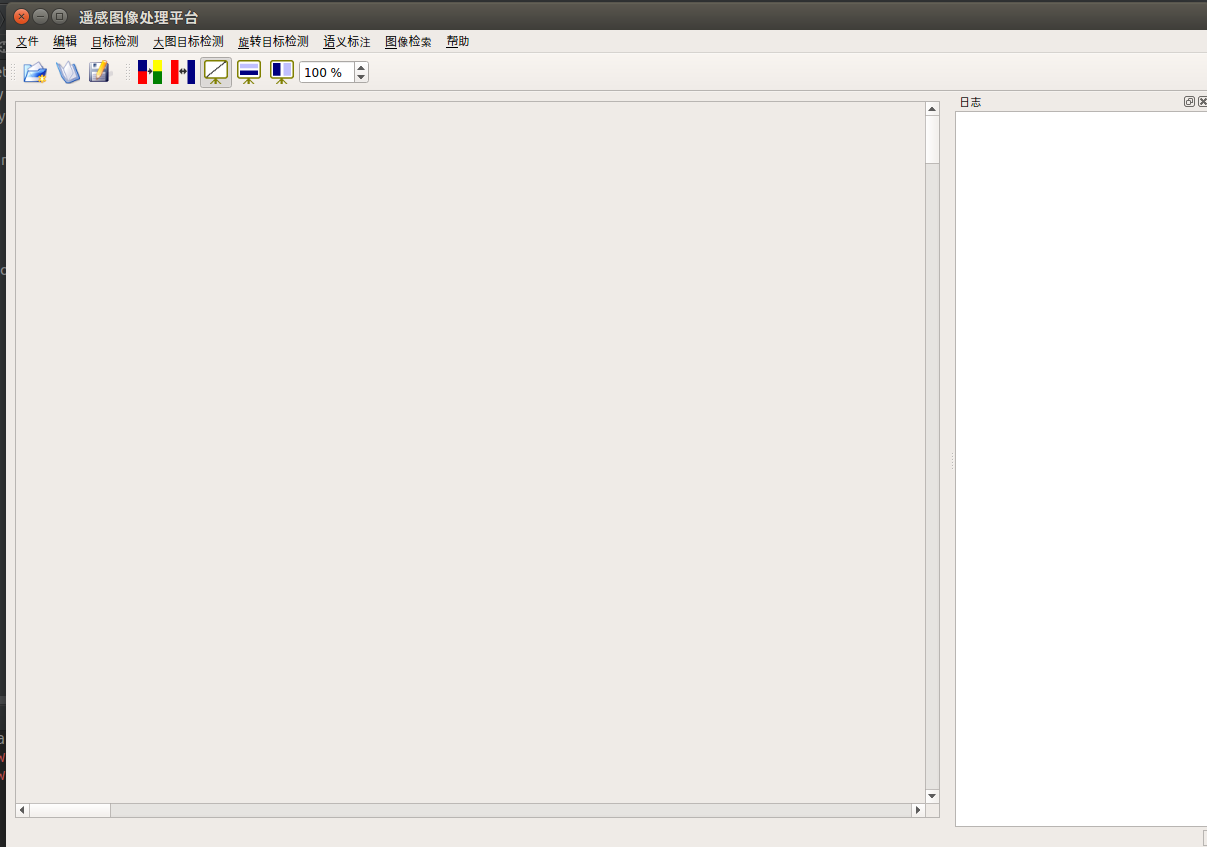
\includegraphics[width=\columnwidth]{full}
				%		 Create a subtitle for the figure.
			\caption{Main page}
			\label{fig:mp}
		    \hspace{0.5cm}
			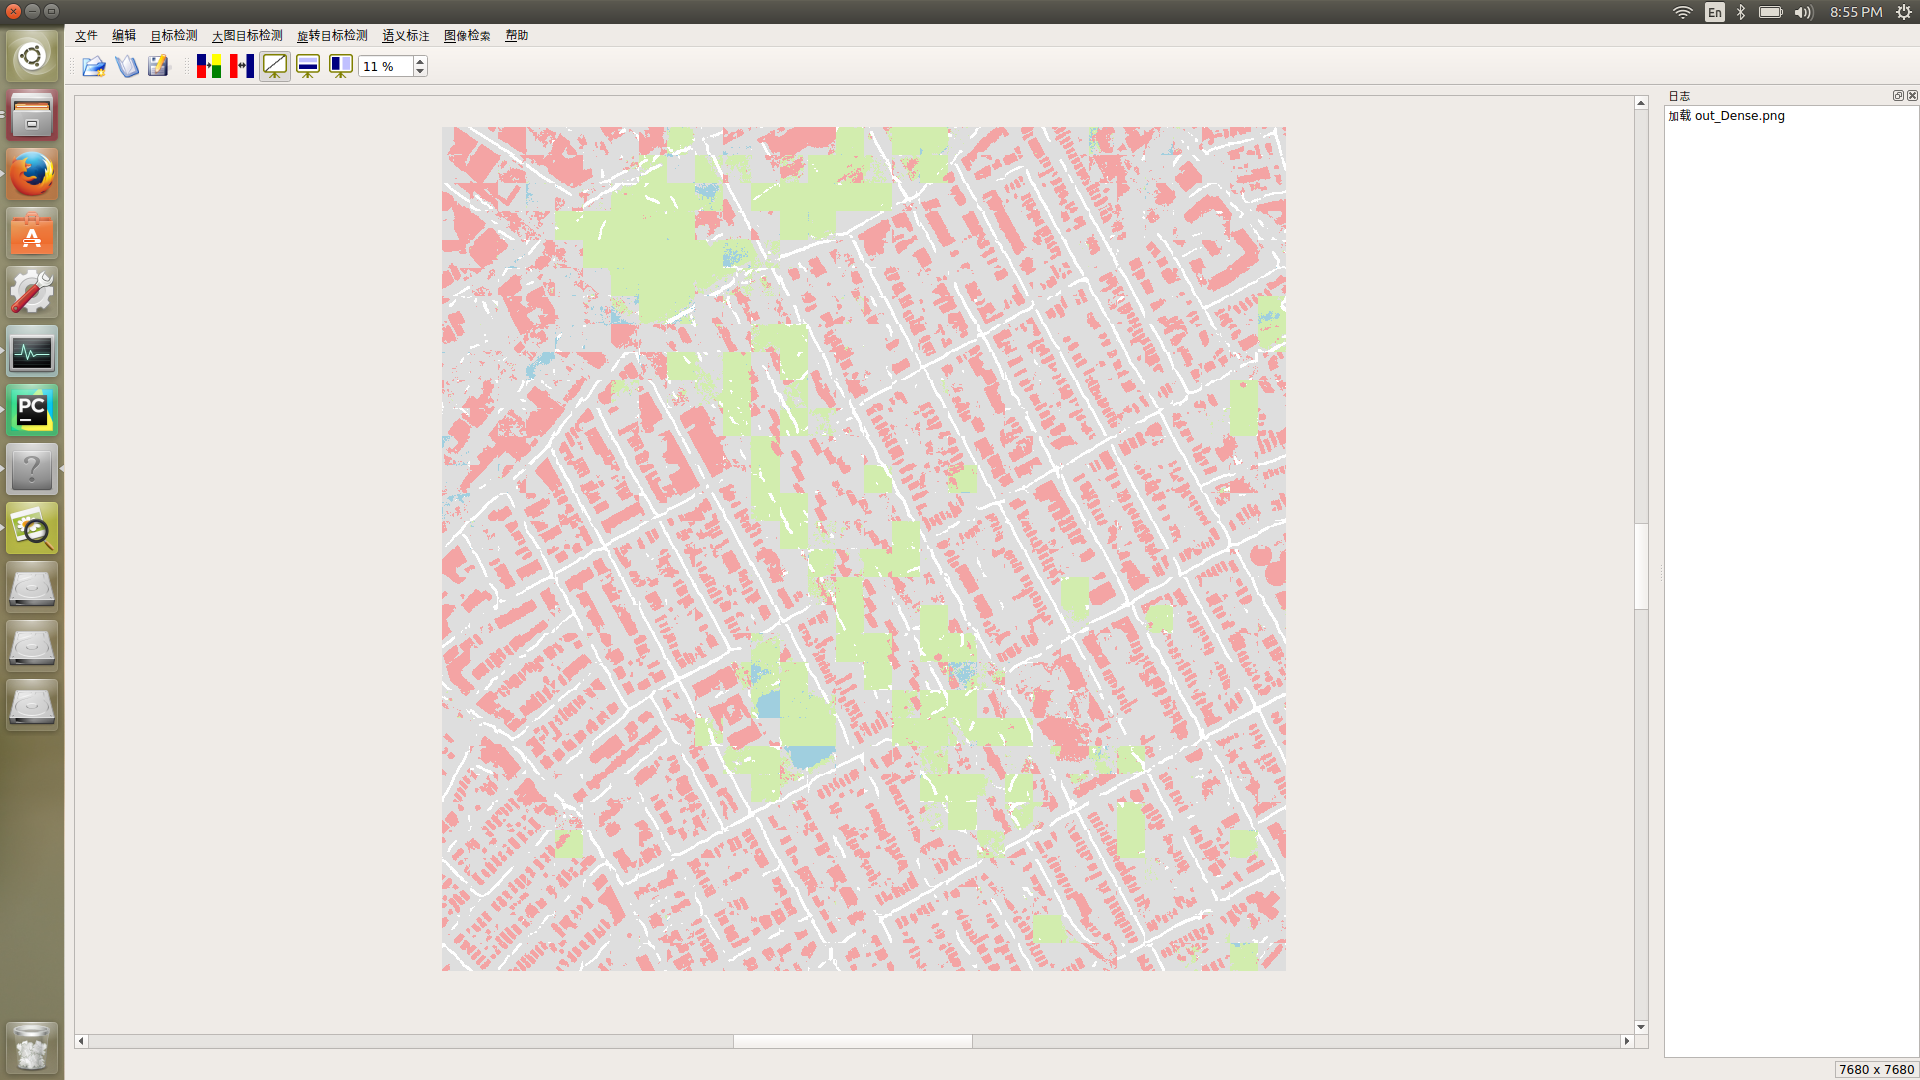
\includegraphics[width=\columnwidth]{ss}
				%Create a subtitle for the figure.
			\caption{Semantic segmentation module}
			\label{fig:ss}
		\end{center}
	\end{figure}

% Now we need a bibliography:
%\begin{thebibliography}{5}
%
%	%Each item starts with a \bibitem{reference} command and the details thereafter.
%	\bibitem{HOP96} % Transaction paper
%	J.~Hagenauer, E.~Offer, and L.~Papke. Iterative decoding of binary block
%	and convolutional codes. {\em IEEE Trans. Inform. Theory},
%	vol.~42, no.~2, pp.~429–-445, Mar. 1996.
%
%	\bibitem{MJH06} % Conference paper
%	T.~Mayer, H.~Jenkac, and J.~Hagenauer. Turbo base-station cooperation for intercell interference cancellation. {\em IEEE Int. Conf. Commun. (ICC)}, Istanbul, Turkey, pp.~356--361, June 2006.
%
%	\bibitem{Proakis} % Book
%	J.~G.~Proakis. {\em Digital Communications}. McGraw-Hill Book Co.,
%	New York, USA, 3rd edition, 1995.
%
%	\bibitem{talk} % Web document
%	F.~R.~Kschischang. Giving a talk: Guidelines for the Preparation and Presentation of Technical Seminars.
%	\url{http://www.comm.toronto.edu/frank/guide/guide.pdf}.
%
%	\bibitem{5}
%	IEEE Transactions \LaTeX and Microsoft Word Style Files.
%	\url{http://www.ieee.org/web/publications/authors/transjnl/index.html}
%
%\end{thebibliography}

% Your document ends here!
\end{document}